%----------------------------------------------------------------------------
\chapter{Evaluation}
%----------------------------------------------------------------------------
This chapter presents the applicability of the designed framework, evaluates its current capabilities and points out improvement possibilities. Section \ref{sec_theoeval} evaluates the current state of the framework, then Section \ref{sec_casestudy} presents a case study about the applicability of our solution. Lastly, Section \ref{sec_futurework} presents the opportunities for the continuation of the work.

%----------------------------------------------------------------------------
\section{Theoretical Evaluation} \label{sec_theoeval}
%----------------------------------------------------------------------------

%----------------------------------------------------------------------------
\section{Case Study: Pedestrian Crossing} \label{sec_casestudy}
%----------------------------------------------------------------------------
This section demonstrates the capabilities and boundaries of the framework. It presents a problem commonly modeled using state-based models, which is complex enough to demonstrate all aspects of the designed Interactive Learning Entity, but also simple enough to solve - thus verify - only using some background knowledge and common sense. [TODO ref gamma tutorial?]

%---------------------------------------------------------------
\subsection{Introduction} \label{subs_casestudyintro}
%---------------------------------------------------------------

The problem to solve is modeling a pedestrian crossing with a standard traffic light and a pedestrian light as illustrated on Figre [TODO]. As the traffic lights and the pedestrian lights on the opposite sides of the crossing behave identically, we are going to model only one instance of each device. 

The traffic light is looping through the red-green-yellow-red sequence. As an extra, there is an interrupted mode that may be triggered by the police, which results in blinking yellow light. The pedestrian light loops through the red-green-red sequence, and turns black when an interrupt arrives. A subsequent interrupt turns the lights back on, also considering that the sytem must always be in a safe state - i.e. the lights must not allow passage for both the pedestrians and the road vehicles at the same time.

The possible states of the imagined system are presented on Figure \ref{fig_casestudy_systemstates}.

\begin{figure}[!ht] 
	\centering
	\fbox{
		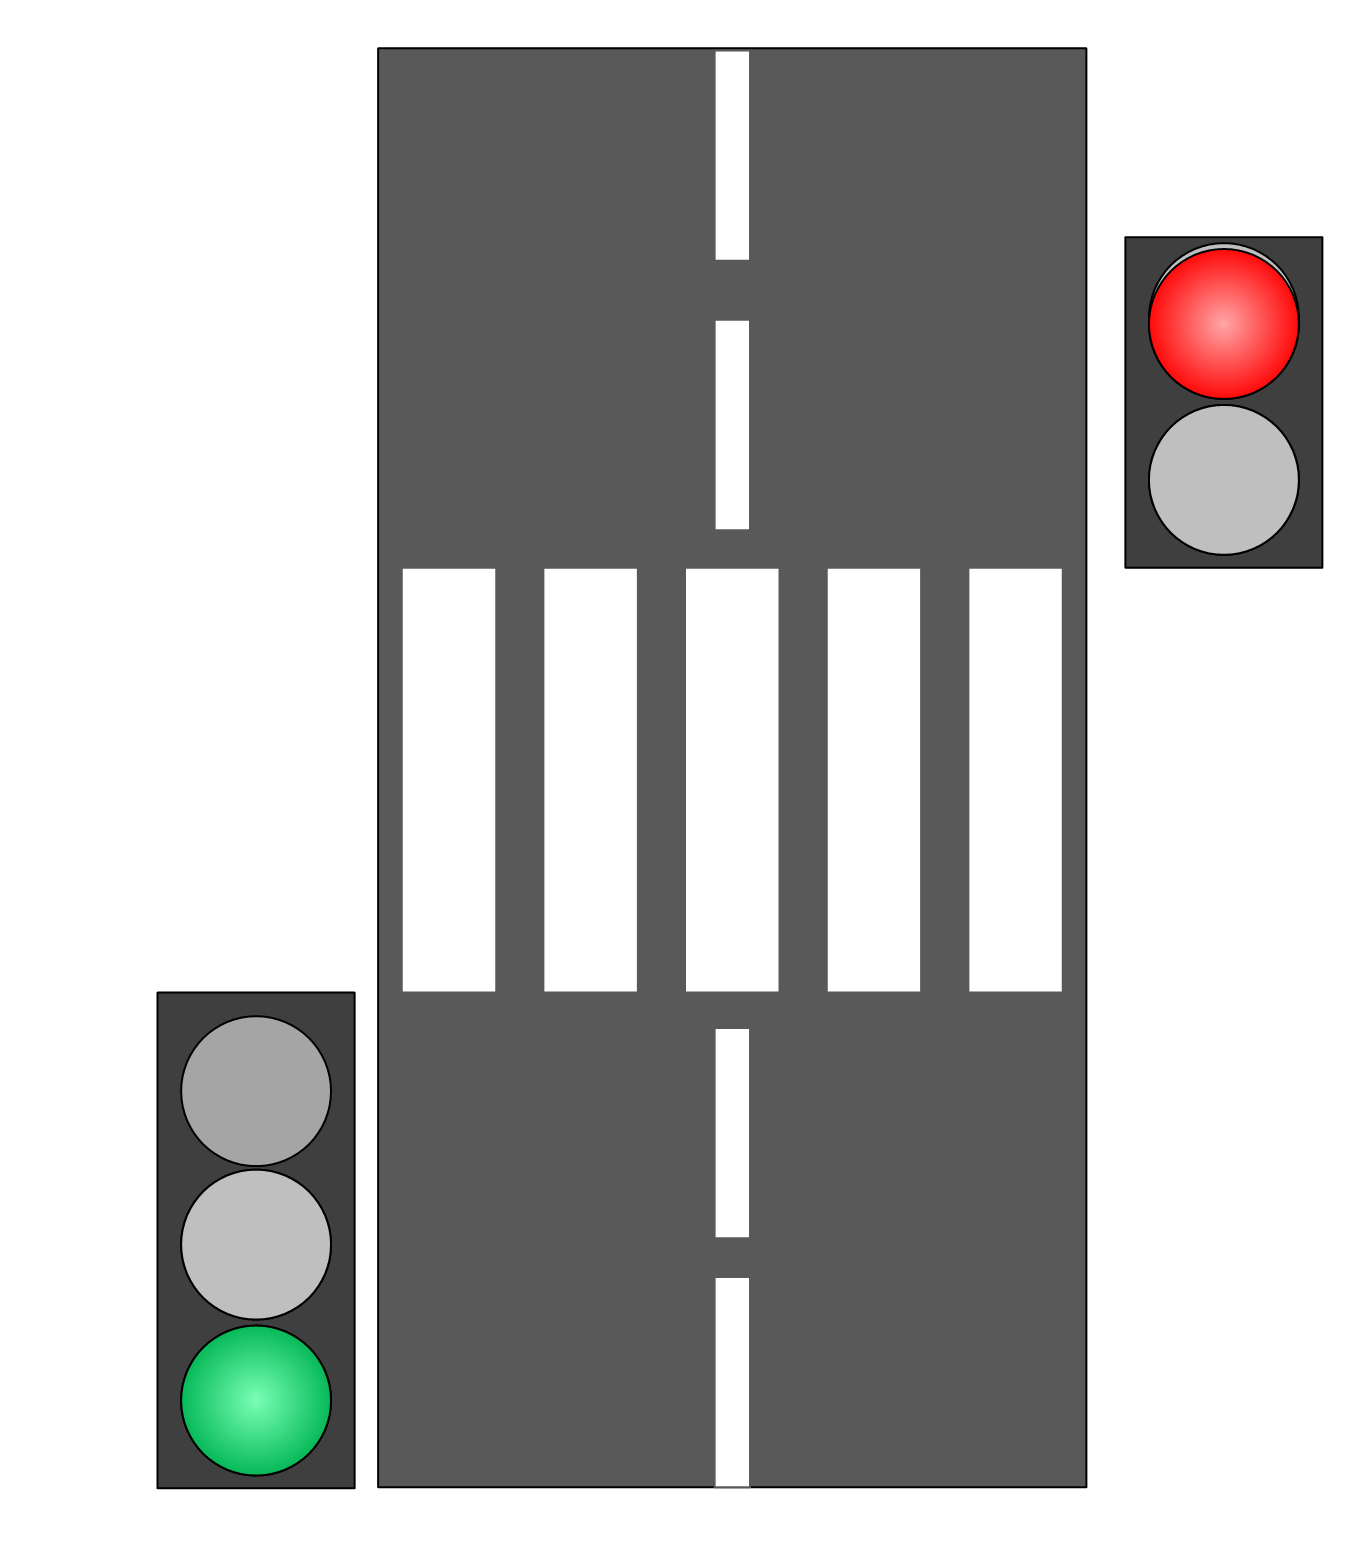
\includegraphics[width=30mm, keepaspectratio]{figures/casestudy_state1.png}
	}
	\fbox{
		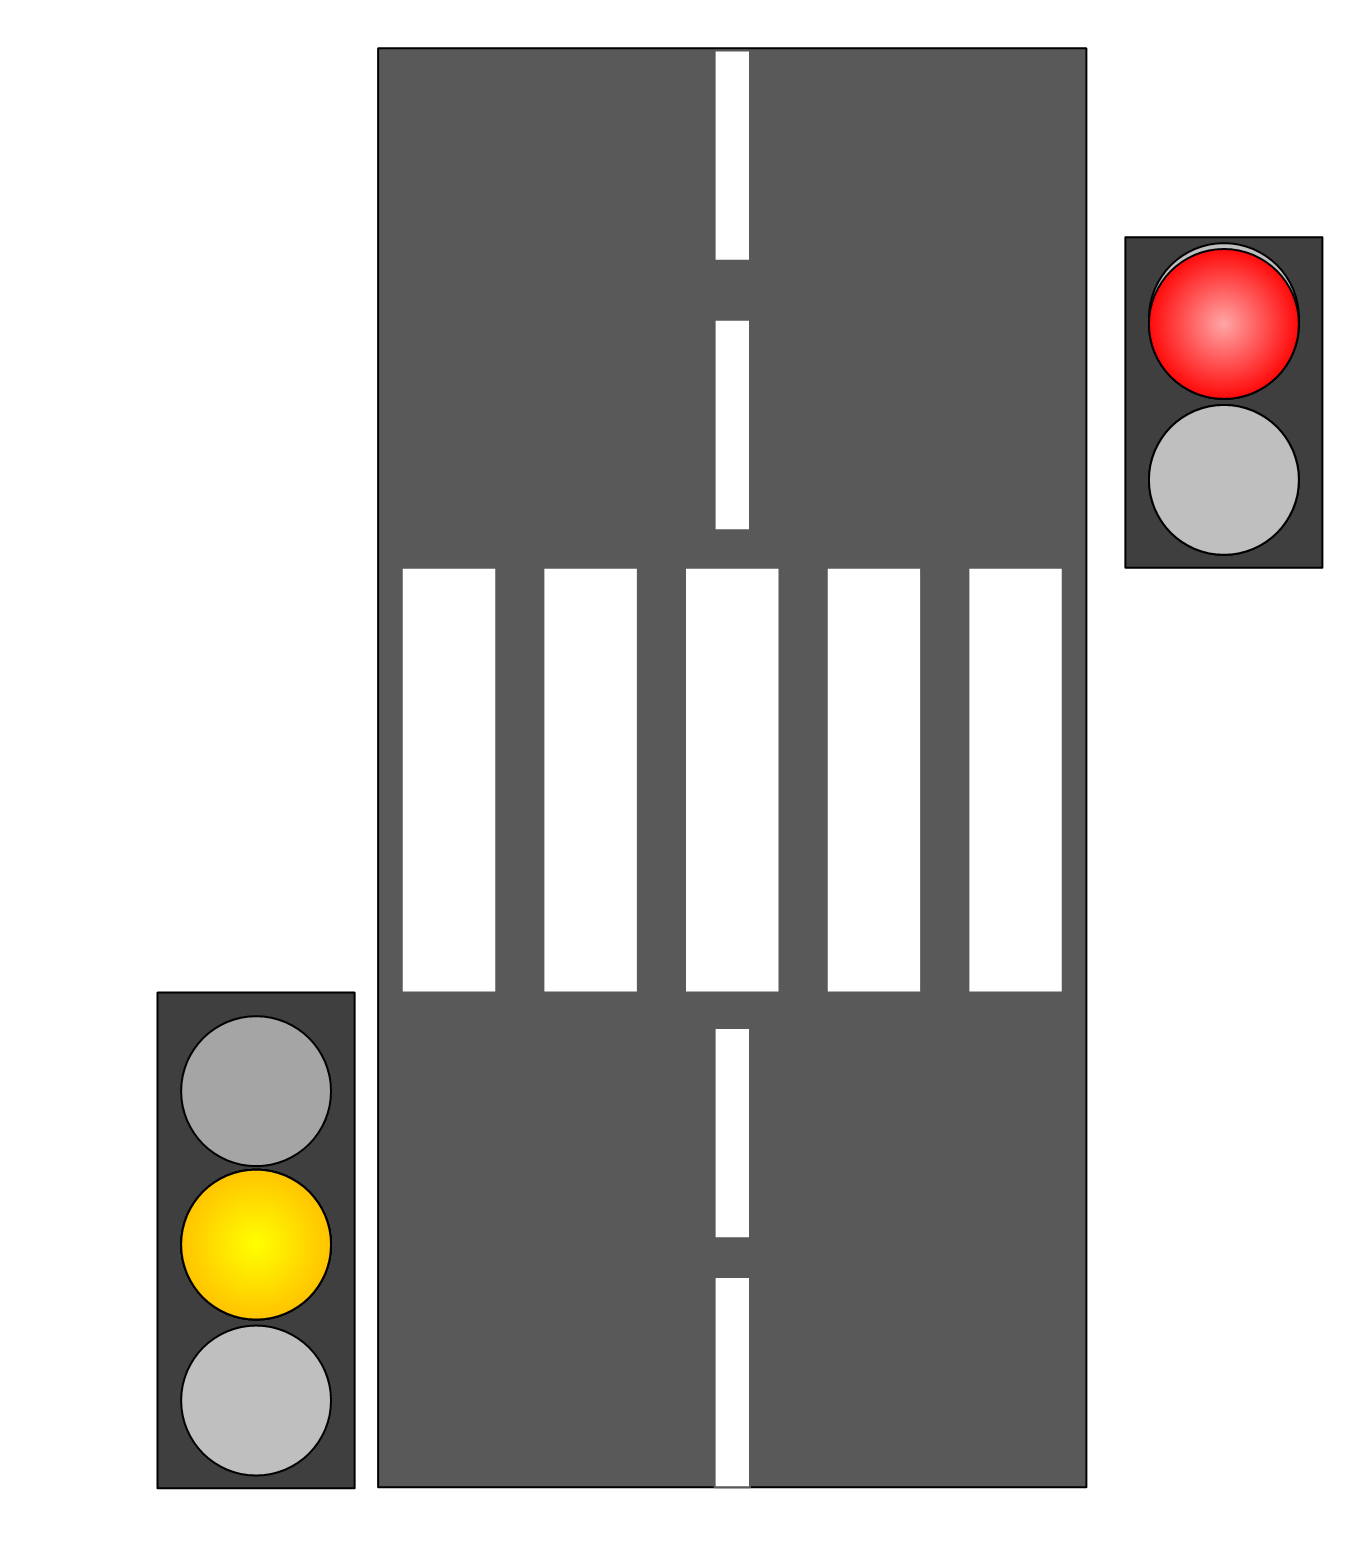
\includegraphics[width=30mm, keepaspectratio]{figures/casestudy_state2.png}
	}
	\fbox{
		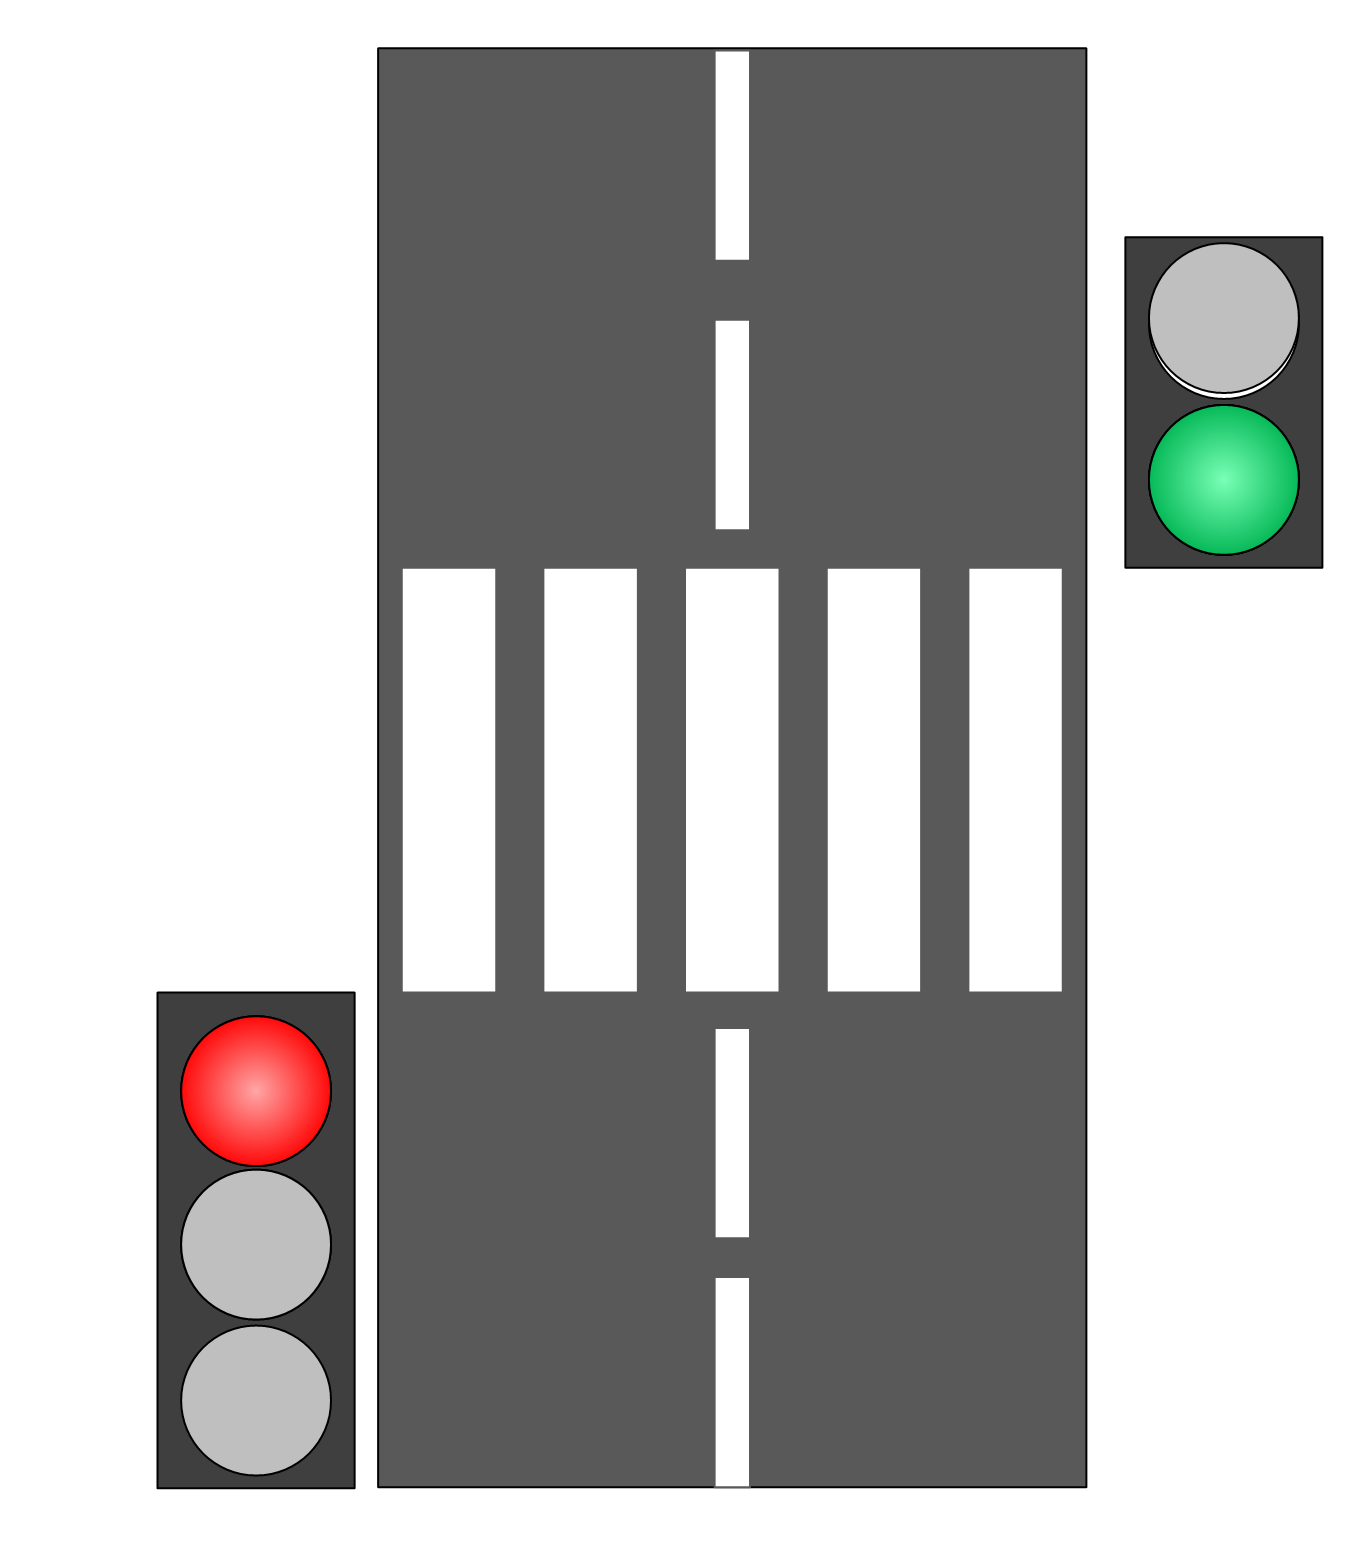
\includegraphics[width=30mm, keepaspectratio]{figures/casestudy_state3.png}
	}
	\fbox{
		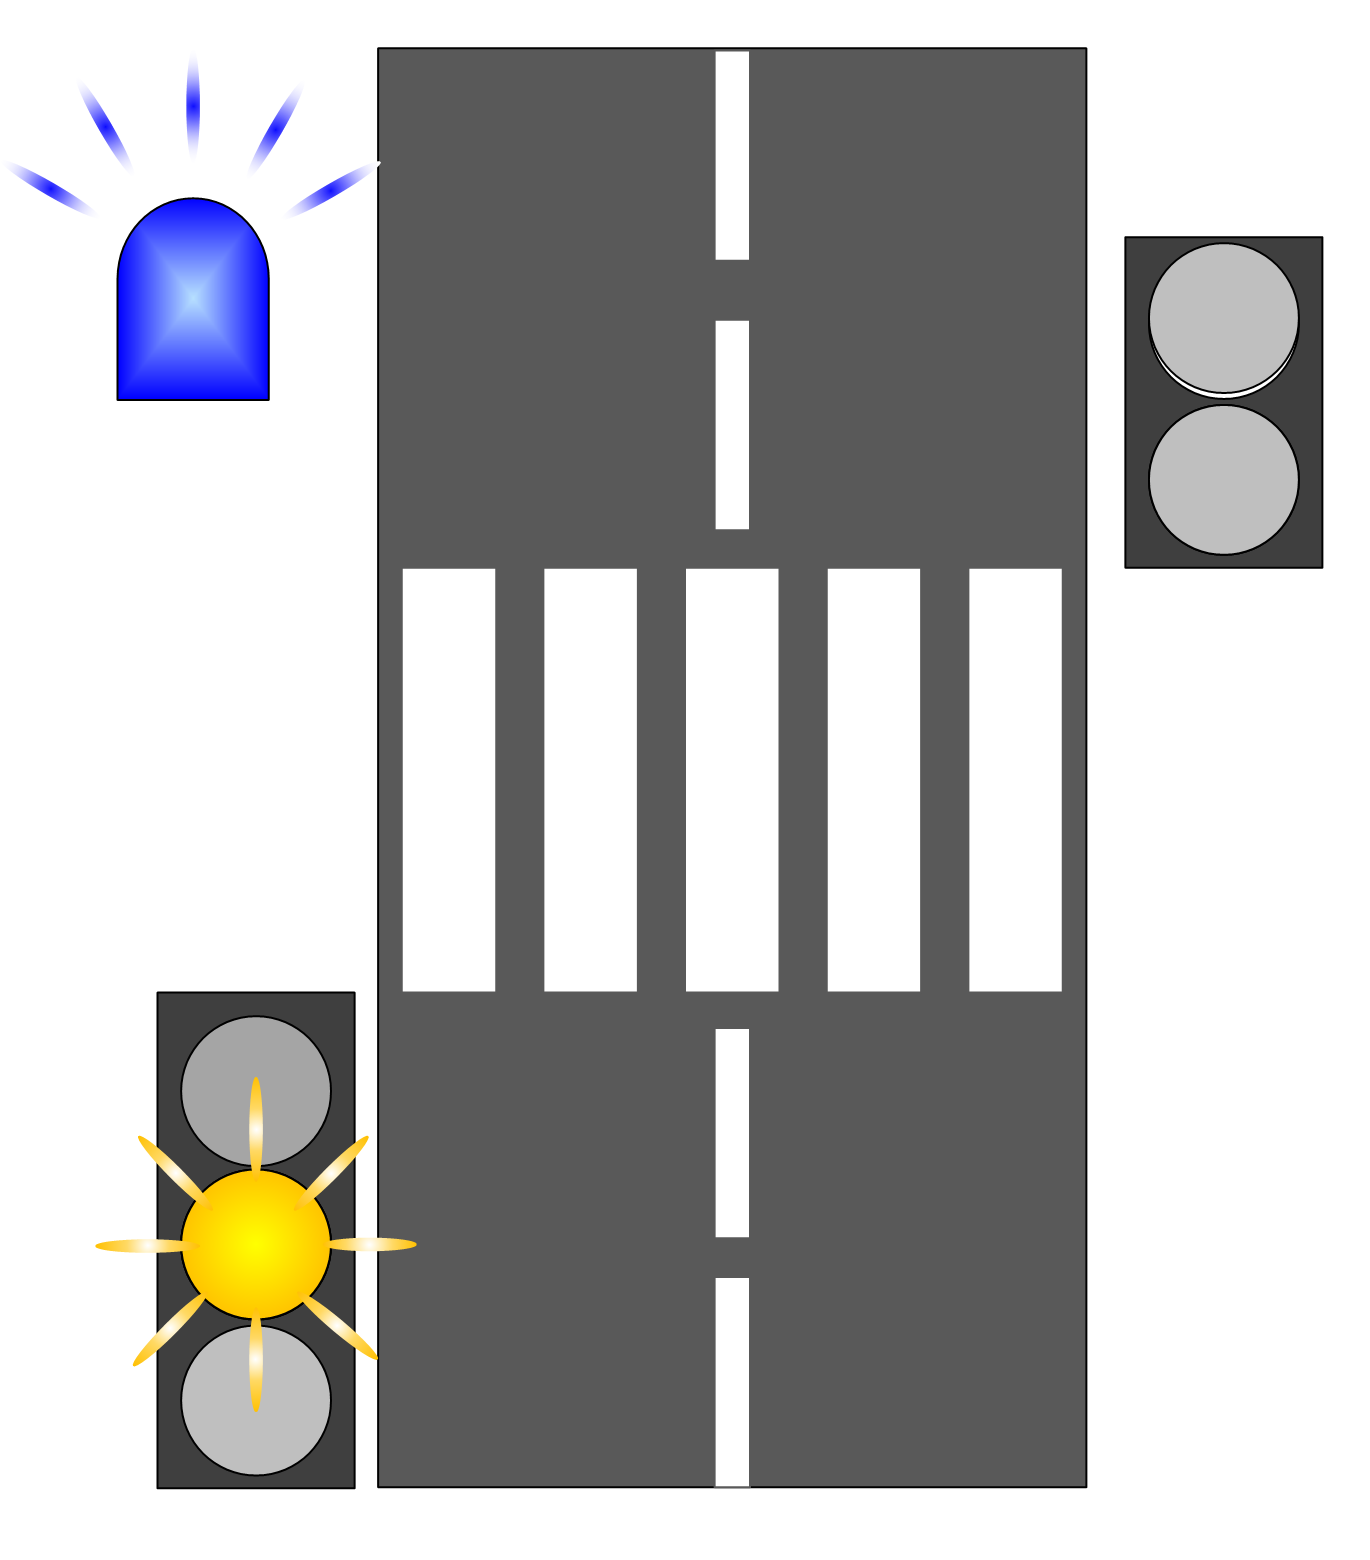
\includegraphics[width=30mm, keepaspectratio]{figures/casestudy_state4.png}
	}
	\caption{Possible states of the system: normal operation (\textit{three from the left}) and the interrupted state \textit{(right)}} 
	\label{fig_casestudy_systemstates}
\end{figure}

%---------------------------------------------------------------
\subsection{Component Design} \label{subs_casestudycomps}
%---------------------------------------------------------------

The previous subsection mentioned two components of the composite system: a traffic light and a pedestrian light. To realize the safe state of the system, the components must synchronize their behavior, justificating the existence of a third, controller component. 

\textbf{The traffic light component} has two inputs on its input interface - toggle and interrupt - and four outputs on its display interface - red, green, yellow and blinking yellow - as it appeared in the problem description.

\textbf{The pedestrian light component} has the same two inputs on its input interface - toggle and interrupt - and three outputs on its display interface - red, green, and black - as it appeared in the problem description.

\textbf{The controller component} controls the rhythm of the change of states and also interrupts the other components when the police interrupt arrives. Thus, it has an input interface for the police interrupt and two output interfaces - matching the inputs of the other components.

The described components and their connections are illustrated on Figure \ref{fig_casestudy_blockdiagram}.

\begin{figure}[!ht] 
	\centering
	%\fbox{
		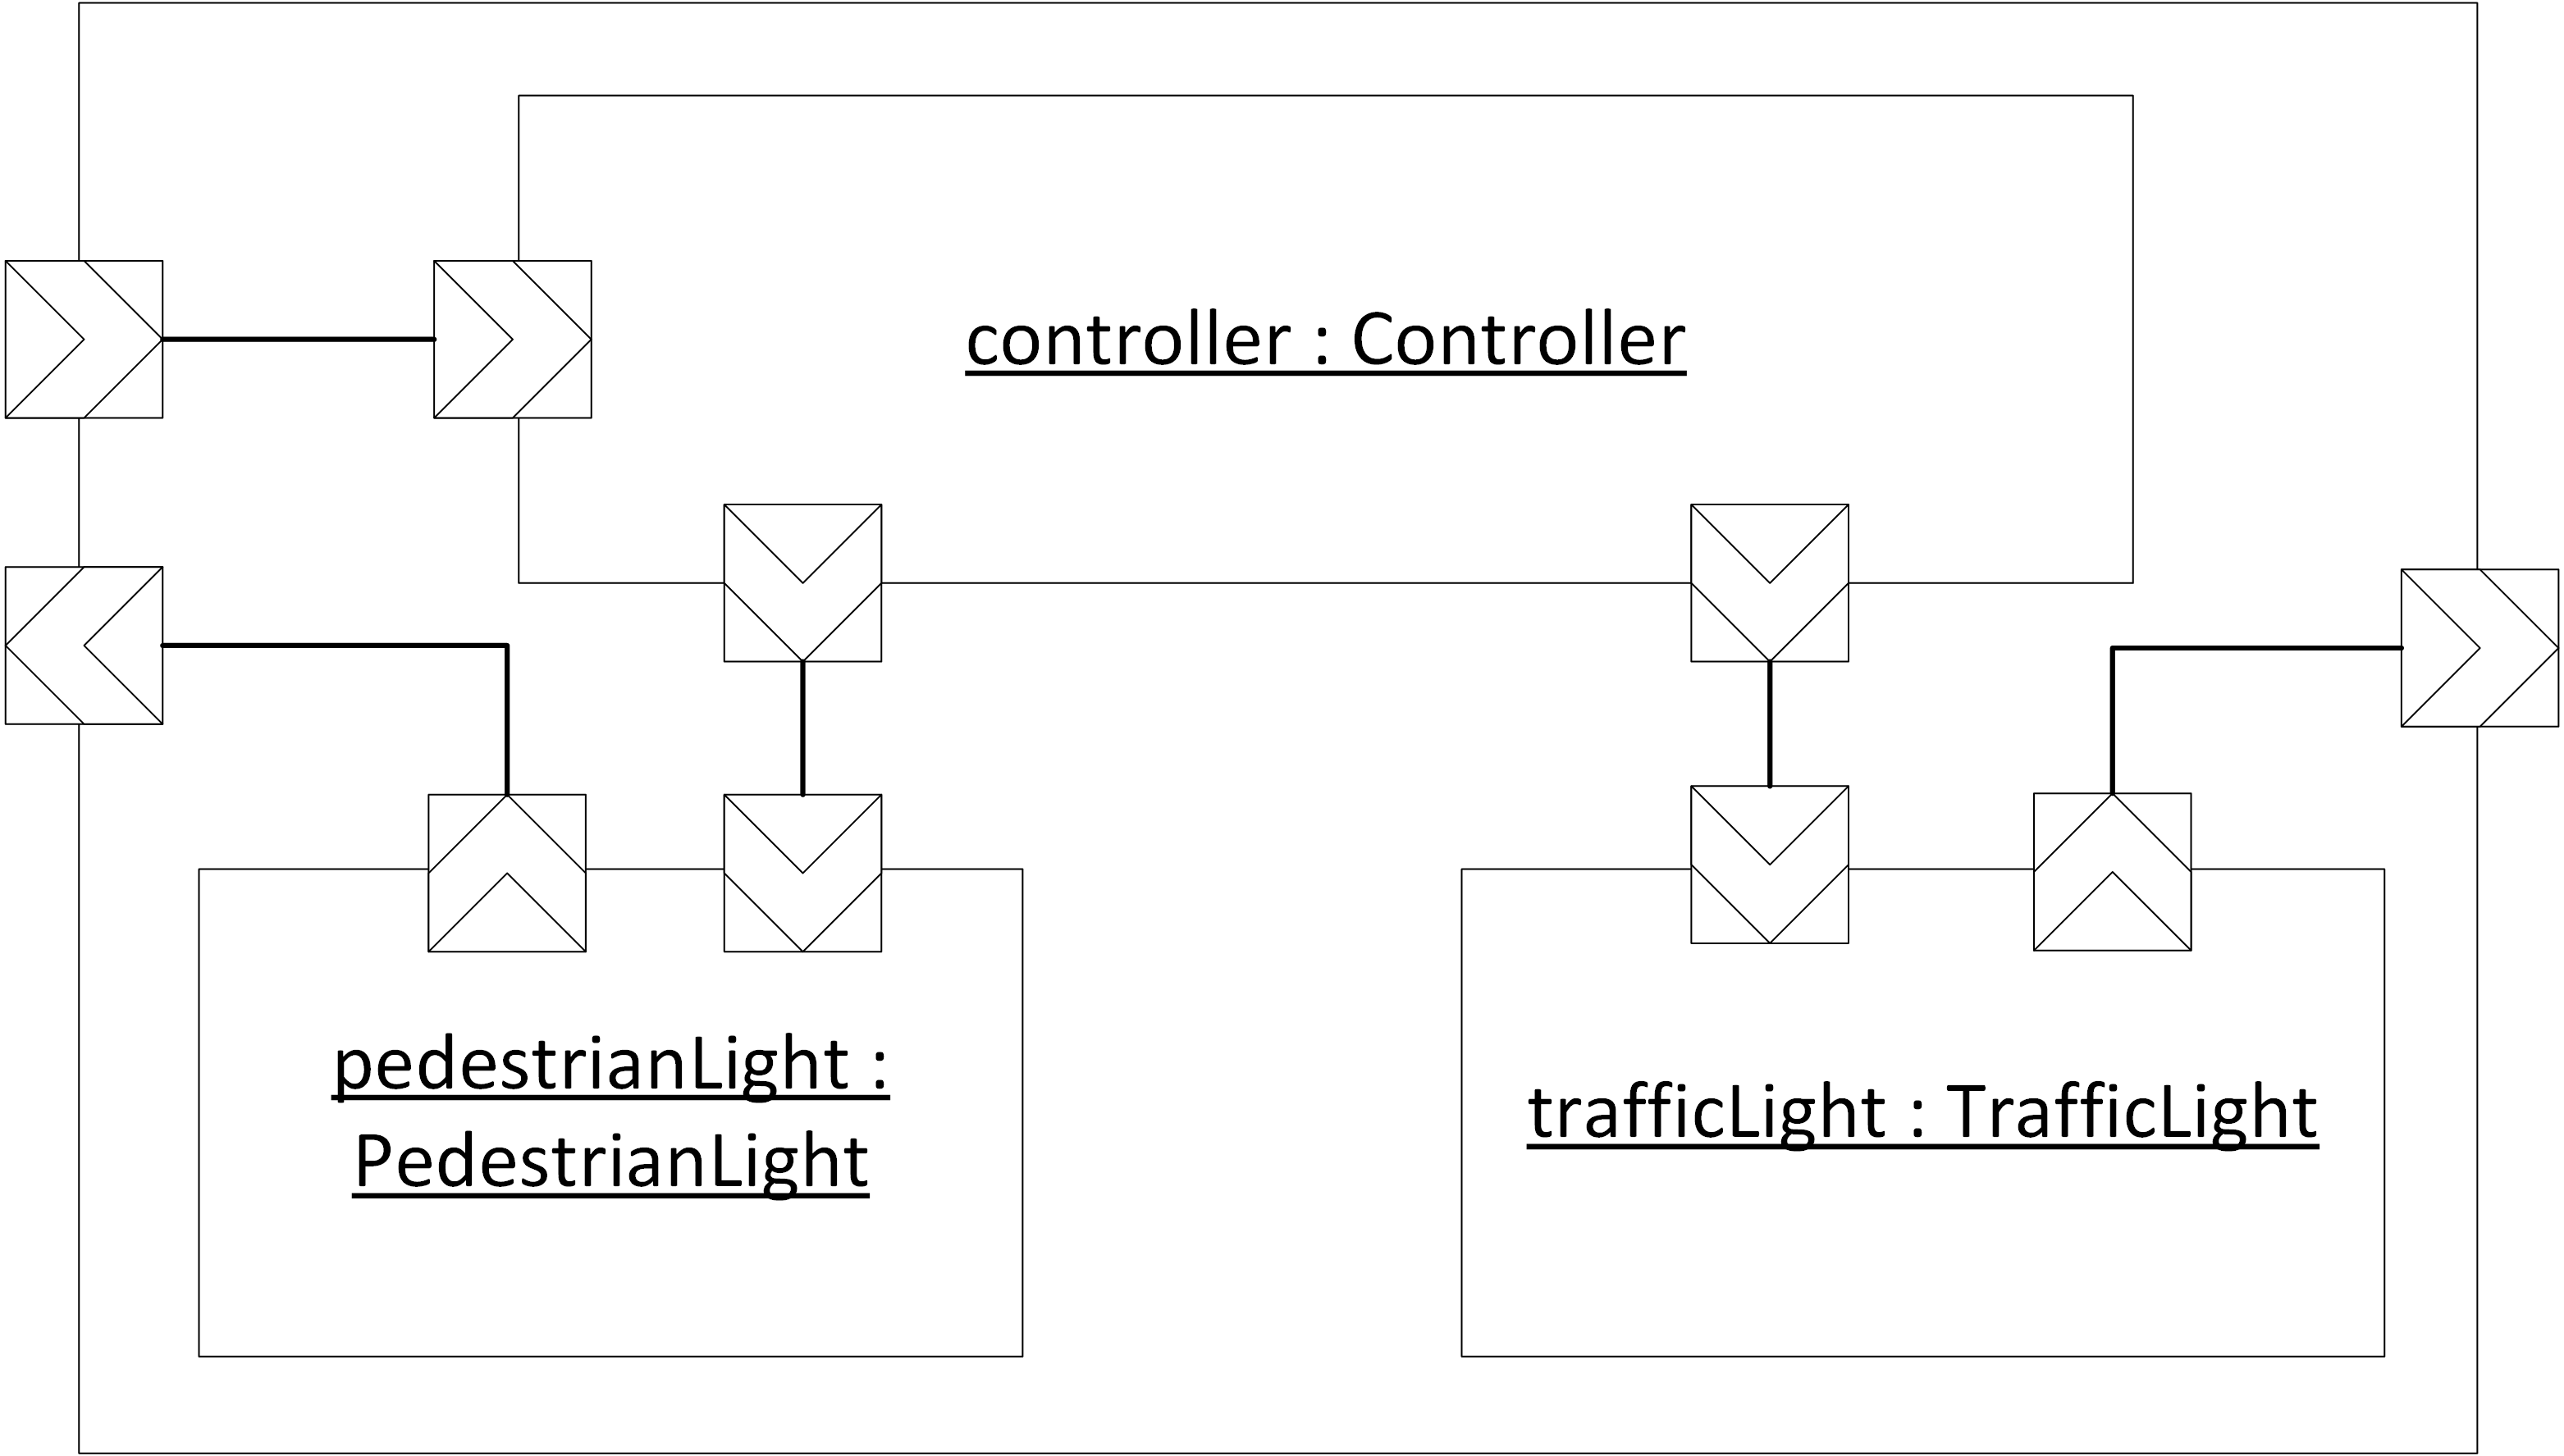
\includegraphics[width=130mm, keepaspectratio]{figures/casestudy_blockdiagram.png}
	%}
	\caption{Components of the modeled system and their connections} 
	\label{fig_casestudy_blockdiagram}
\end{figure}

%---------------------------------------------------------------
\subsection{Synthesizing a Component Using the Framework} \label{subs_casestudysynth}
%---------------------------------------------------------------

%---------------------------------------------------------------
\subsection{The Resulting System} \label{subs_casestudyresults}
%---------------------------------------------------------------


%----------------------------------------------------------------------------
\section{Future Work} \label{sec_futurework}
%----------------------------------------------------------------------------

